\documentclass[11pt,a4paper]{article}
\usepackage{graphicx}
\usepackage{amssymb}
\usepackage[slovene]{babel}
\usepackage[utf8]{inputenc}
\usepackage[backend=bibtex, style=ieee]{biblatex}

\bibliography{ciites} 
\title{Vpliv poravnave na uspešnost razpoznavanja uhljev}
\author{Dispozicija diplomske naloge\\
\ \\
Kandidat: Metod Ribič \\
\ \\
Mentor: izr. prof. dr. Peter Peer\\
\ \\
Fakulteta za računalništvo in informatiko\\
\ \\
Univerza v Ljubljani}
\date{\today}                                          



\begin{document}
\maketitle

\section{Kratek opis podro\v{c}ja in delovne hipoteze}

Diplomsko delo sodi na področje računalniškega vida, natančneje na področje biometrije uhljev, kjer z obliko uhljev poskušamo razpoznati osebo, podobno kot to že vrsto let uspešno počnemo s prstnimi odtisi. Algoritmi razpoznave ter poravnave uhljev sicer obstajajo, ampak jih je potrebno prilagoditi oziroma spremeniti do te mere, da bodo delovali na bazi uhljev AWE \cite{earsReview2016}. Slike so majhnih ločljivosti, zato imajo ti algoritmi problem, ker imajo majhno površino za pridobivanje značilk. Rezultati diplomske naloge bi morali prikazati izboljšan odstotek razpoznave oseb na podlagi poravnanih uhljev v primerjavi z neporavnanimi uhlji.


\section{Cilj diplomske naloge}

Cilj te diplomske naloge je zgraditi ter v uporabo ponuditi poravnano bazo uhljev, s pripadajočimi rezultati v primerjavi z neporavnano bazo uhljev, ter vključiti kodo, ki vodi do teh rezultatov v orodje AWE. Orodje je poleg baze uhljev prosto za uporabo.


\section{Metodolo\v ski pristop}

V svoji diplomski nalogi bom uporabil naslednja metodološka pristopa:
\begin{itemize}
	\item Pregled podro\v cja -- na tem področju je raziskanih ter opisanih že veliko rešitev za točno določeno 						problematiko, sam bom preučil nekaj ključnih postopkov ter izpostavil morebitne pomanjkljivosti oziroma težave v povezavi z AWE bazo uhljev.
	\item Primerjalna \v studija -- preučil bom več metod povezanih s poravnavo, ter ovrednotil, katera od njih oziroma katera kombinacija teh doprinese najboljši rezultat.

\end{itemize}

\section{Miselni vzorec}

Na sliki~\ref{fig:miselni_vzorec} miselni vzorec prikazuje postopek poravnave ter kasnejše obdelave rezultatov v orodju AWE.

\begin{figure}[p]
    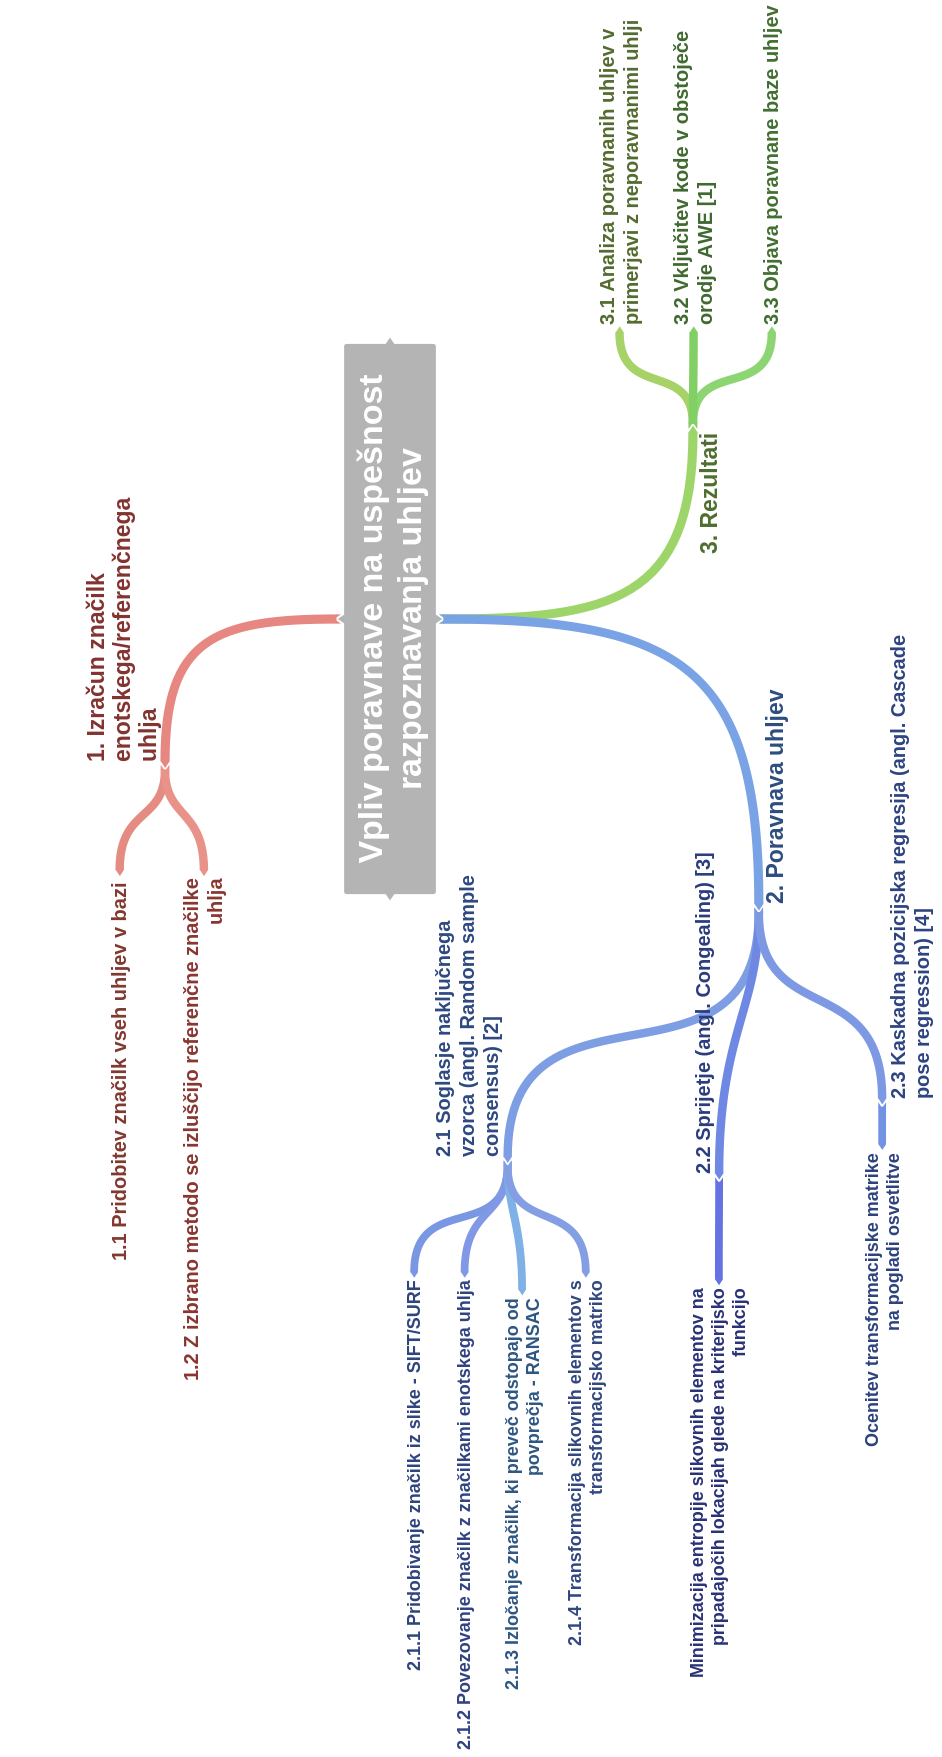
\includegraphics[scale=0.345]{diagram_final}
    \caption{Miselni vzorec poteka poravnave uhljev.}
    \label{fig:miselni_vzorec}
\end{figure}


\section{Okvirno kazalo diplome}

\begin{enumerate}
\item Uvod
\item Orodja in knjižnice
\item Opis metod in postopkov
\begin{enumerate}
		  	\item{Izračun značilk referenčnega uhlja}
          \item{Soglasje naključnega vzorca \emph{(angl. RANSAC)} \cite{fischler1981random}}
          \item{Sprijetje \emph{(angl. Congealing)} \cite{huang2007unsupervised}}
          \item{Kaskadna pozicijska regresija \emph{(angl. Cascaded Pose Regression)} \cite{pflug2015ear}} 
\end{enumerate}
\item Eksperimenti
\item{Rezultati z diskusijo}
\item{Zaklju\v cek}
\end{enumerate}

\section{Temeljna literatura}

\printbibliography

\end{document}  